% Camera-based weather-severity estimation for adaptive driving under fog and rain in MetaDrive.
% Every number in Sections VI-VII is copied from measured files:
%   bev_rl/adaptive/results/severity_eval_20seed_snapshot (120 episodes, SHA-256 manifest)  -> severity_eval_20seed_analysis/summary.json
%   bev_rl/adaptive/results/severity_estimator/eval_heldout.json
%   bev_rl/adaptive/results/teacher_identity_caution/*.json
%   bev_rl/adaptive/results/camera_dagger_severity/e2e_sevB/train_round*.json
% Extension results (seeds 5220-5239) are marked EXTENSION and are filled in when available.
\documentclass[conference]{IEEEtran}
\IEEEoverridecommandlockouts
\usepackage{cite}
\usepackage{amsmath,amssymb,amsfonts}
\usepackage{graphicx}
\usepackage{booktabs}
\usepackage{array}
\usepackage{textcomp}
\usepackage{xcolor}
\usepackage{tikz}
\usetikzlibrary{positioning,arrows.meta,fit,calc}
\usepackage[hidelinks]{hyperref}
\newcommand{\todo}[1]{\textcolor{red}{[TODO: #1]}}
\newcommand{\chat}{\hat{c}}
\DeclareMathOperator*{\argmax}{arg\,max}

\begin{document}

\title{Adapting a Camera-Driven Policy to Fog and Rain from Image-Estimated Weather Severity:\\
Energy Savings and an Unresolved Clear-Weather Failure in MetaDrive}

\author{\IEEEauthorblockN{Author 1, Author 2, Author 3, Author 4}
\IEEEauthorblockA{Department of Computer Science and Engineering, PES University, Bengaluru, India\\
Guide: Prof.\ Guide Name}}

\maketitle

\begin{abstract}
We study whether a camera-driven driving policy can adapt its behaviour to weather using only the image itself. A lightweight estimator maps seven global statistics of a front camera frame to a weather kind (clear, fog, rain) and a per-kind intensity, which a temporal filter turns into a scalar caution $\chat\in[0,1]$. A driving policy that receives this scalar through a small branch is trained by DAgger through the complete camera pipeline (five RGB cameras, stereo depth, a detector, a bird's-eye-view builder) from a privileged teacher whose target speed and following gap depend on caution. We compare this adaptive policy (Model C) with a non-adaptive policy from the same pipeline (Model A) on 20 paired MetaDrive scenarios per condition, under identical weather noise, with traction energy computed from the speed trace. On held-out routes the estimator reaches a macro recall of $0.979$ and mean absolute errors of $0.045$ (fog) and $0.051$ (rain), with no false caution in clear weather. In severe fog and rain, Model C succeeded in 20 of 20 episodes in both, as Model A did, and reduced the paired traction energy per kilometre by $48.9\%$ (fog) and $48.7\%$ (rain) with speeds of about $5.5$\,m/s instead of $7.8$\,m/s. In clear weather, however, Model C succeeded in 17 of 20 episodes against 20 of 20 for Model A: two stalls and one early collision, all with correct zero caution, and no significant energy difference. The adaptation is therefore effective under severe synthetic weather, while preserving clear-weather performance remains unresolved. The evaluation is pilot-scale, simulation-only, and uses synthetic image-space weather.
\end{abstract}

\begin{IEEEkeywords}
adaptive driving, weather severity estimation, imitation learning, DAgger, energy-aware driving, MetaDrive
\end{IEEEkeywords}

%==============================================================================
\section{Introduction}
Fog and rain degrade what a camera-based driver can perceive, and human drivers respond by driving more slowly and keeping larger gaps. A learned driving policy that ignores weather either drives as in clear conditions, which is unsafe when perception is impaired, or is trained to be uniformly conservative, which wastes time and energy when the weather is fine. We ask a narrower question than weather classification: can the \emph{driving behaviour} itself be made to depend on the severity of weather, estimated from the camera image alone, and what does this do to success, collisions and energy?

We build one system and measure it end to end (Fig.~\ref{fig:arch}): camera images, an image-based severity estimate, a caution score, an adaptive driving policy, and safe driving with energy measurement. The emphasis is on the \emph{outcome} of adaptation in closed loop, not on the accuracy of a weather classifier.

\textbf{Contributions.}
\begin{enumerate}
\item An image-based severity estimator that uses no additional sensor: seven statistics of the front camera frame feed a kind classifier and separate fog and rain intensity regressors, followed by a temporal filter. It is evaluated on routes that were never used for fitting.
\item A camera-in-the-loop adaptive policy. The policy receives the filtered caution through a dedicated input branch (indirect conditioning: it never sees a weather label), and is trained by DAgger through the full camera pipeline against a privileged, caution-aware teacher. The same network is run with the oracle caution during training and with the image-estimated caution at inference (a plug-in design).
\item A traction-energy formulation for MetaDrive speed traces (inertial, aerodynamic and rolling work per step, no regeneration), whose assumptions are declared, and which is used to report paired Wh/km next to success and collisions.
\item A paired, instrumented evaluation of the adaptive and a non-adaptive policy under fog, rain and clear weather, with an honest report of a failure mode: the adaptive policy fails in clear weather where the non-adaptive policy does not.
\end{enumerate}

%==============================================================================
\section{Related Work}
\textbf{Simulators and learned driving.} MetaDrive provides procedurally generated, composable driving scenarios for reinforcement and imitation learning~\cite{li2022metadrive}. Imitation learning with on-policy relabelling (DAgger)~\cite{ross2011dagger} is the standard remedy for the compounding error of behaviour cloning, and privileged-teacher approaches train a sensor-based student from a teacher with access to simulator state~\cite{chen2019cheating,zhang2021roach}. ChauffeurNet showed that plain cloning of expert driving is insufficient without augmentation~\cite{bansal2019chauffeurnet}. We follow the privileged-teacher, DAgger recipe, and the teacher relabels only the states the student visits.

\textbf{Perception and driving under adverse weather.} Fog and rain degrade camera perception, and surveys document the effects on detection, depth and localisation~\cite{zhang2023adverse}. Synthetic fog is commonly generated from a depth-based attenuation model~\cite{sakaridis2018foggy}, and image corruptions provide standard robustness benchmarks~\cite{hendrycks2019corruptions}. Most of this literature improves perception robustness. Our setting differs: perception is left as it is, and the \emph{policy} is made to adapt its behaviour to an estimate of how bad the weather is.

\textbf{Safe speed given limited visibility.} Formal safety models derive a maximum safe speed and following distance from the perception range and the reaction time~\cite{shalev2017rss}, and microscopic car-following models such as the Intelligent Driver Model~\cite{treiber2000idm} relate speed to gap. Our teacher uses an IDM-style car-following rule whose desired speed and gap are functions of a caution value, which is a design choice and not a visibility-derived bound.

\textbf{Energy.} Vehicle traction energy is commonly modelled from longitudinal dynamics: inertial, aerodynamic and rolling-resistance work~\cite{guzzella2013propulsion}. We apply this model to MetaDrive speed traces, because the simulator has no usable energy model for our purpose (Section~\ref{sec:energy}).

\textbf{Perception stack.} The camera pipeline uses semi-global stereo matching~\cite{hirschmuller2008sgm} and a YOLO detector~\cite{redmon2016yolo,jocher2023yolov8}.

%==============================================================================
\section{Problem Formulation}
\label{sec:problem}
\textbf{Environment.} An episode is a sequence of decisions at $10$\,Hz in a MetaDrive scenario with sparse traffic (density $0.05$). At step $t$ the ego vehicle has five camera images $I_t^{(j)}$, $j=1,\dots,5$, that have passed through a weather intervention
\begin{equation}
\tilde I_t^{(j)} = W\big(I_t^{(j)};\,k,\ell,\xi_t\big),\qquad k\in\{\text{clear},\text{fog},\text{rain}\},\ \ell\in[0,1],
\end{equation}
where $\xi_t$ is a noise draw that depends only on the scenario seed and the step, so that two policies evaluated on the same seed see identical weather noise. The weather $(k,\ell)$ is fixed within an episode and is unknown to the policy.

\textbf{Perception and state.} A frozen pipeline $\Phi$ turns the weathered images into a $64\times64$ bird's-eye-view (BEV) grid $b_t=\Phi(\{\tilde I_t^{(j)}\})$. The policy also receives six ego scalars $s_t$. It receives \emph{no} simulator position.

\textbf{Caution.} We define the true caution by the identity mapping
\begin{equation}
c(k,\ell)=\begin{cases}0 & k=\text{clear},\\ \ell & k\in\{\text{fog},\text{rain}\}.\end{cases}
\label{eq:caution}
\end{equation}
This is a design assumption, not a claim of physical equivalence: fog and rain levels are normalised inside their own generators, and equal numbers do not mean equal visibility or danger. The estimator produces $\chat_t\approx c(k,\ell)$ from the front-left frame alone.

\textbf{Policies.} A policy $\pi_\theta(a_t\mid b_t,s_t,\gamma_t)$ outputs steering and throttle/brake $a_t\in[-1,1]^2$. Model A has no caution input ($\gamma_t$ absent). Model C uses $\gamma_t=\chat_t$. During training the same network is given $\gamma_t=c$ (the oracle value); we call this network trained with oracle caution Model~B, and use it only as a training reference. Model C is Model B's network with $\gamma_t=\chat_t$ at inference.

\textbf{Objective.} Let $S$ be success (route completed without collision, leaving the road or timing out), $U$ a collision or off-road event, and $e$ the traction energy per kilometre (Section~\ref{sec:energy}). The goal is to reduce $e$ in adverse weather without reducing $S$ or increasing $U$, and without changing behaviour in clear weather:
\begin{align}
\min_\theta\ & \mathbb E[e \mid k\!\neq\!\text{clear}] \quad\text{s.t.}\quad \Pr(S)\ge \Pr(S_A)-\delta,\\
& \Pr(U)\le \Pr(U_A)\ \text{in adverse weather},\quad \bar v_{\text{clear}}\approx \bar v_A,
\end{align}
where $A$ denotes Model~A and $\delta=0.10$ is used descriptively. The paired estimand for energy is
\begin{equation}
\Delta_e = \mathbb E\big[e_C - e_A \,\big|\, S_A=S_C=1\big],
\end{equation}
over scenarios in which both policies succeed, with all-episode energies reported separately.

%==============================================================================
\section{Methodology}
\subsection{Weather intervention}
Weather acts on each camera picture only (image space, no depth dependence). With intensity $\ell$: \emph{fog} blends each row towards white with a weight that increases linearly from $0$ at the top row to $0.9\,\ell$ at the bottom row, then applies Gaussian blur and additive noise whose strength grows with $\ell$; \emph{rain} adds $\lfloor 800\ell\rfloor$ bright streaks, blurs and blends them, and darkens the image by a fixed $25\%$ at all levels. The two front pictures receive an identical noise draw so stereo matching is not corrupted independently. Because the filter is image-space and level-normalised, it has no extinction coefficient, so physics-based visibility estimators do not apply (Section~\ref{sec:limits}).

Figure~\ref{fig:frames} shows front-camera frames under the four weather settings (illustrative frames from earlier runs of the same scene).
\begin{figure*}[t]
\centering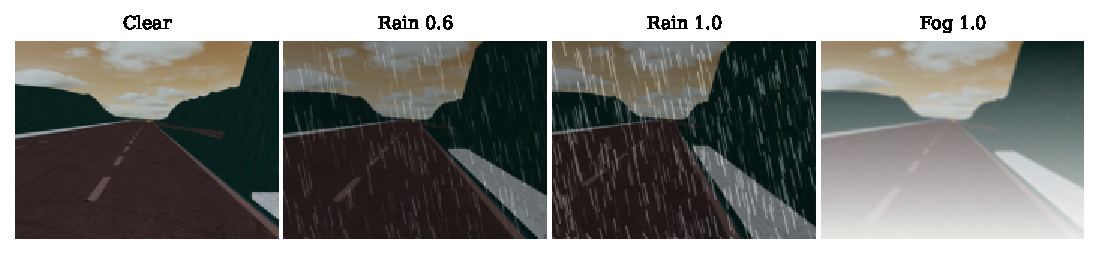
\includegraphics[width=0.85\textwidth]{figures/fig_weather_frames.pdf}
\caption{Front-camera frames after the weather intervention: clear, rain $0.6$, rain $1.0$ and fog $1.0$ (same scene, illustrative).}\label{fig:frames}
\end{figure*}

\subsection{Image-based severity estimation}
\label{sec:estimator}
\textbf{Features.} From the final weather-processed front-left frame (computed at quarter scale) we compute $x\in\mathbb R^7$: log Laplacian variance, mean gradient magnitude, RMS contrast, mean dark channel, brightness, saturation, and the share of strong edges. These are the features of a visibility sensor that already existed in the pipeline, which we reuse unchanged.

\textbf{Kind and intensity.} With standardised features $\tilde x$, a softmax classifier
\begin{equation}
\hat p=\operatorname{softmax}(W\tilde x+b)\in\Delta^2
\end{equation}
(balanced class weights, $\ell_2$ penalty $10^{-2}$) predicts the kind, and per-kind ridge regressors (penalty $1$)
\begin{equation}
\hat\ell_k=\operatorname{clip}\big(w_k^\top\tilde x+b_k,\,0,\,1\big),\qquad k\in\{\text{fog},\text{rain}\},
\end{equation}
estimate intensity, each fitted on clear frames (level $0$) plus frames of its own kind. Hyper-parameters were fixed before any held-out data was examined.

\textbf{Temporal filter.} The kind probabilities are smoothed, $q_t=(1-\alpha_p)q_{t-1}+\alpha_p\hat p_t$, the kind is $\hat k_t=\argmax q_t$, and the per-frame level $\hat\ell_t=0$ if $\hat k_t=\text{clear}$ and $\hat\ell_{\hat k_t}$ otherwise is smoothed,
\begin{equation}
\chat_t=(1-\alpha_c)\,\chat_{t-1}+\alpha_c\,\hat\ell_t,\qquad \alpha_p=\alpha_c=0.15 .
\end{equation}

\textbf{Estimator data.} The estimator is fitted on $25{,}408$ frames: every step of the whole-route DAgger episodes (Section~\ref{sec:dagger}; weather levels clear, fog $0.3/0.8/1.0$, rain $0.2/0.6/1.0$) plus $28$ earlier whole-route episodes. Four probe levels (fog $0.45$ and $0.6$, rain $0.3$ and $0.45$) never enter any fit. The held-out set is three independent whole-route episodes (seeds $9040$--$9042$), each rendered under all ten weather conditions.

\subsection{Teacher and caution-aware behaviour}
The teacher is privileged (it reads simulator state) and is used only to label states. It is an IDM-style car-following controller combined with a safety layer and a curve guard (limit $4.0$), whose desired speed and following distance depend on caution:
\begin{equation}
v^\star(c)=\frac{30}{3.6}\Big(1-\frac{c}{3}\Big)\ \text{m/s},\qquad d^\star(c)=10+15c\ \text{m}.
\label{eq:teacher}
\end{equation}
At $c=0$ the target is $8.33$\,m/s and at $c=1$ it is $5.56$\,m/s. Validated on $50$ episodes per condition (seeds $3100$--$3149$, horizon $1600$) with the true caution, the teacher succeeded in $49/50$ (clear), $48/50$ (fog and rain $0.6$) and $49/50$ (fog and rain $1.0$), with mean speeds $7.80$, $6.41$ and $5.41$\,m/s. The teacher sees only $c$, so fog and rain give identical results at equal level.

\subsection{Driving policy}
The policy has a convolutional branch for the BEV grid, a multilayer-perceptron branch for the six scalars, and a caution branch (a fully connected layer $1\to16$). The branch outputs are concatenated into a $176$-dimensional fusion vector followed by a head $176\to128\to2$. Model~A uses the same architecture without the caution branch. Initialisation of the caution network is from an earlier caution-conditioned checkpoint; Model~A's checkpoint was trained earlier by camera DAgger and is not modified.

\subsection{Training by camera-pipeline DAgger}
\label{sec:dagger}
Training follows DAgger~\cite{ross2011dagger}. In round $r$ the data are collected through the complete camera pipeline at every step, the teacher labels the visited state with its clean action $a^\star$, and the student executes either the teacher's action with probability $\beta_r$ ($\beta_0=1$, $\beta_r=0.5^r$) or its own, with Gaussian action noise ($\sigma=0.1$). After each round the network is retrained on all data so far with the mean-squared-error loss
\begin{equation}
\mathcal L(\theta)=\mathbb E_{(o,a^\star)\sim\mathcal D_{\le r}}\,\big\|\pi_\theta(o)-a^\star\big\|^2,
\end{equation}
using Adam (learning rate $10^{-3}$, batch $128$) for $18$ epochs in round $0$ and $6$ afterwards. The student receives the oracle caution $c$. Rounds $0$--$3$ each use $12$ episodes (horizon $600$, density $0.05$) from a balanced list of clear (twice), fog $0.3/0.8/1.0$ and rain $0.2/0.6/1.0$. Cumulative training samples and final losses were $6{,}078$ ($0.0044$), $11{,}616$ ($0.0116$), $17{,}541$ ($0.0047$) and $23{,}532$ ($0.0068$). The final-round network is used; no validation-based checkpoint selection was done (a schedule decision). This is a smaller schedule than the originally planned $40$ episodes per round, because each camera episode costs $10$--$35$ minutes of wall time.

%==============================================================================
\section{System Architecture}
Figure~\ref{fig:arch} shows the complete system. A weather intervention is applied to all five camera images. Two paths start from the same images. The \emph{driving path} (left) extracts objects with stereo depth and a detector, builds a frozen BEV grid with map layers, and adds the ego scalars. The \emph{severity path} (right) computes seven features of the front-left frame, estimates kind and intensity, and filters them into $\chat$. The policy fuses both paths and outputs steering and throttle/brake. The energy meter and outcome logger observe the executed trajectory. The teacher exists only at training time.

\begin{figure}[t]
\centering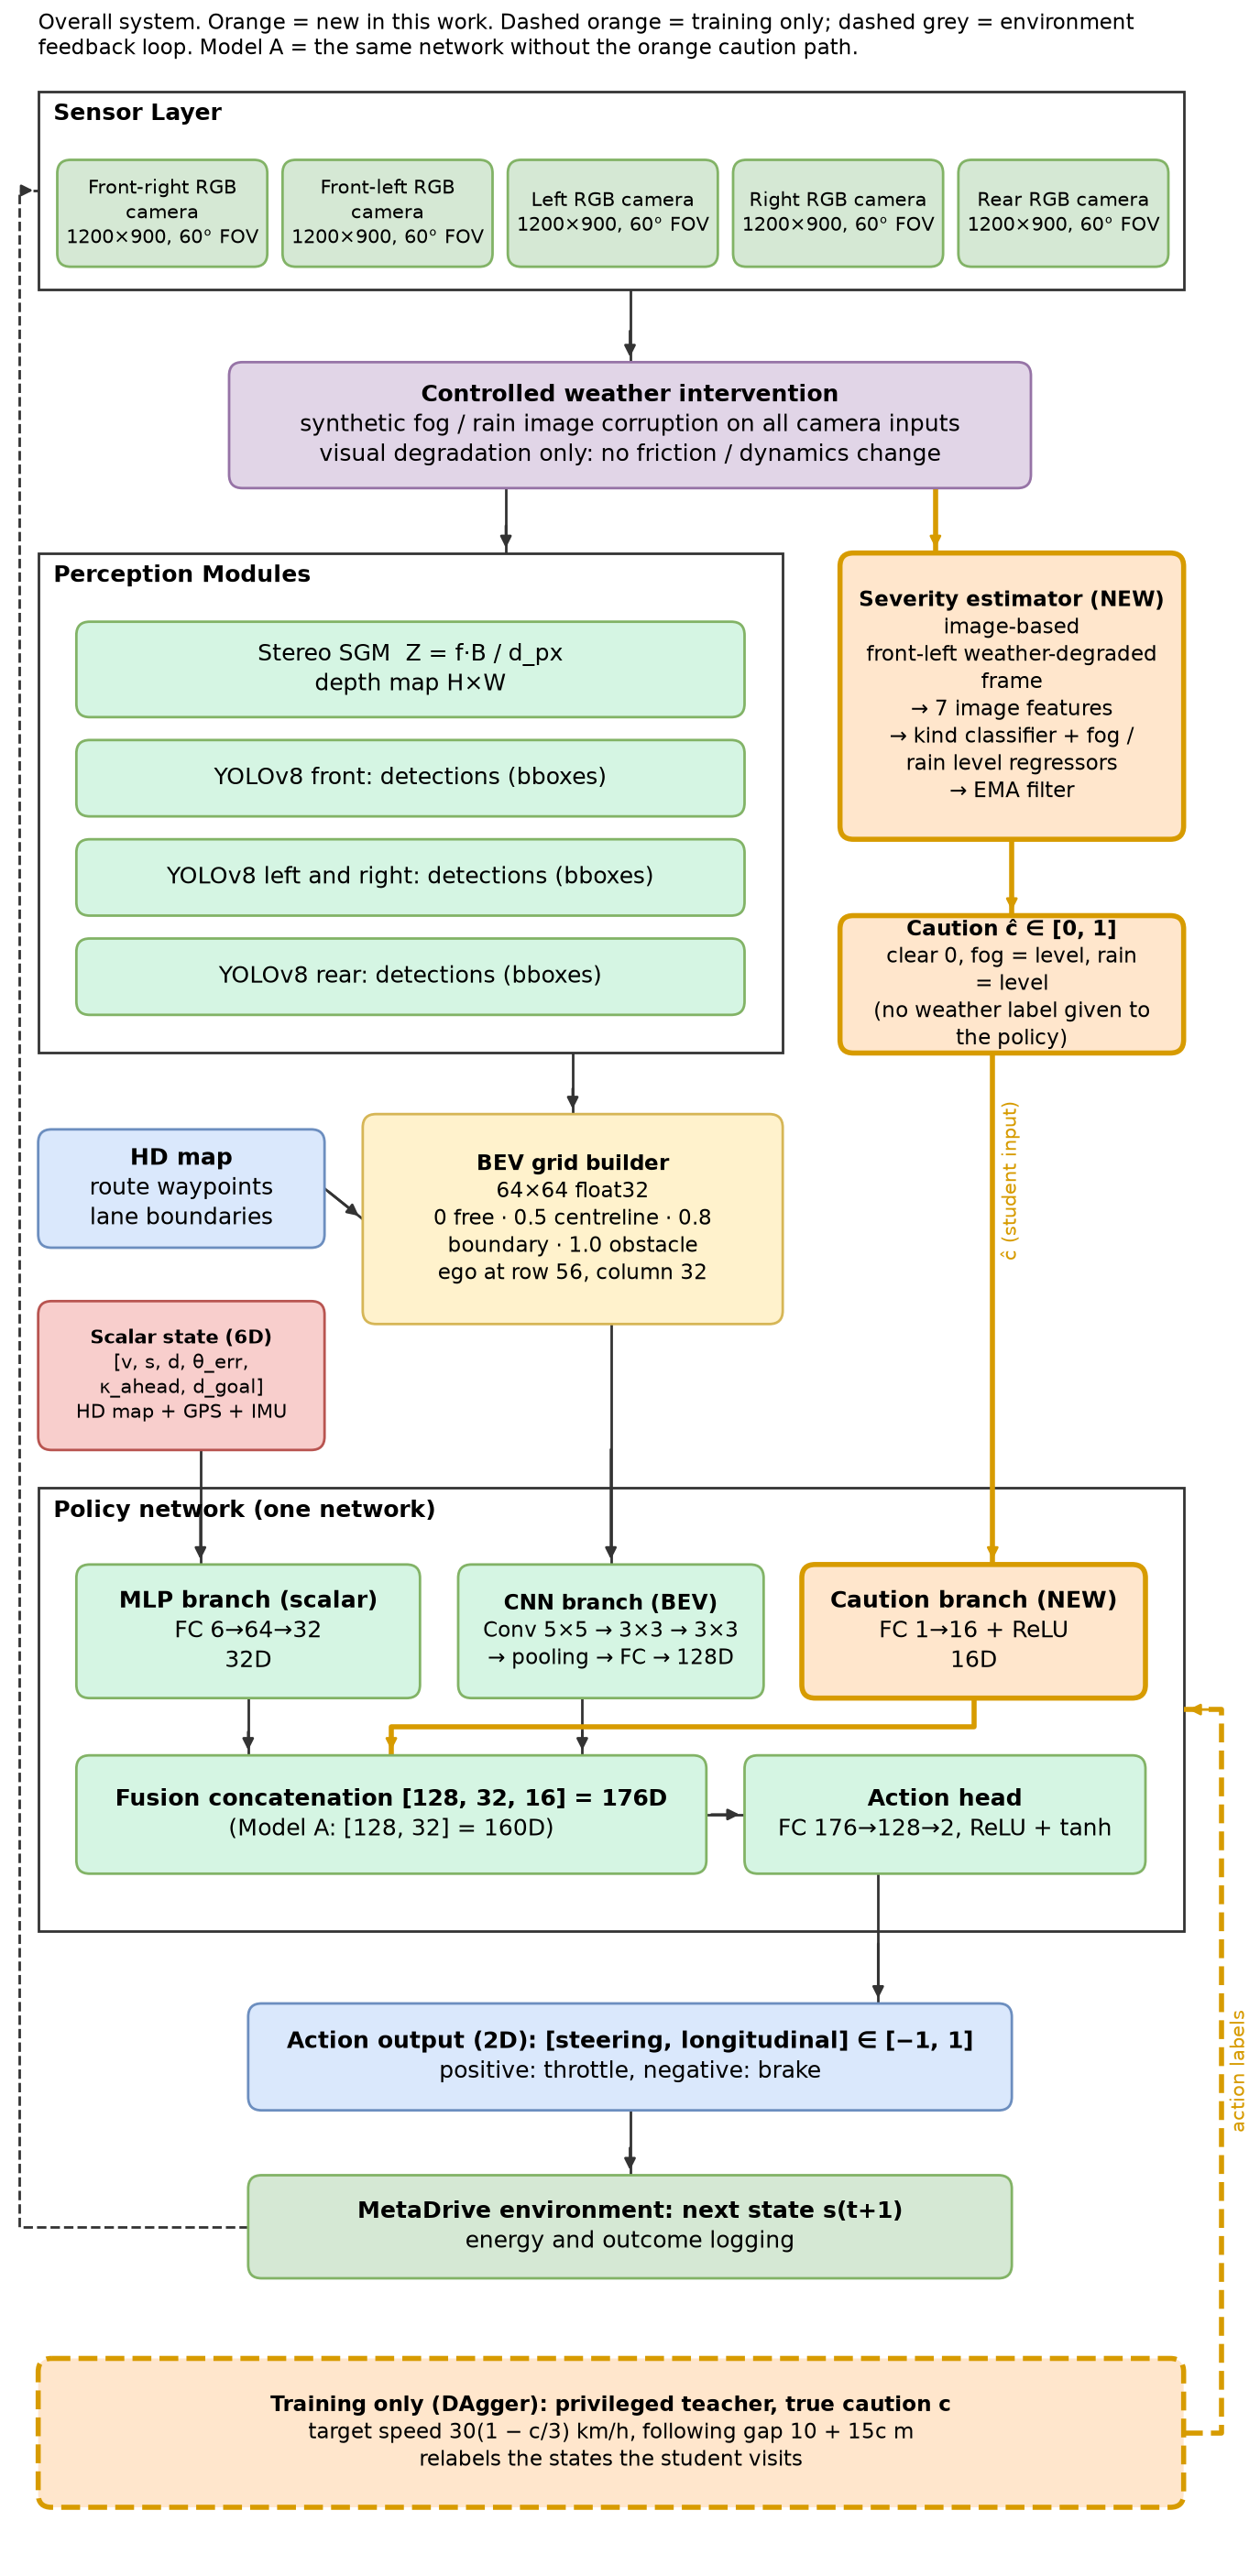
\includegraphics[width=\columnwidth]{figures/fig_architecture.png}
\caption{Overall system (vertical layout). Orange marks what is new in this work: the image-based severity estimator, the caution $\hat c$ and the caution branch of the policy. The dashed box is used only for training. Model~A is the same network without the orange path. Module expansions are in the appendix.}
\label{fig:arch}
\end{figure}

%==============================================================================
\section{Experimental Setup and Evaluation Metrics}
\subsection{Models and conditions}
\textbf{Model A} is the non-adaptive camera policy (no caution input); \textbf{Model C} is the adaptive system. Model~B (oracle caution) is a training reference and was not evaluated for the results reported here. Conditions: clear, fog $1.0$, rain $1.0$. Paired scenario seeds $5200$--$5219$ ($20$ pairs per condition, $120$ episodes), traffic density $0.05$, primary horizon $1600$ steps, no teacher and no action noise at test time. The seeds were never used for training or tuning. Both arms run the same scenario with identical weather noise. The estimator also runs in shadow mode for Model~A, to log $\chat$ against the true caution.

\subsection{Metrics}
\textbf{Primary:} success rate; collision and off-road events; paired Wh/km on pairs where both policies succeeded (with all-episode Wh/km reported separately, because failed episodes cover less distance). \textbf{Secondary:} route completion, mean speed, duration, share of steps with deceleration below $-2$\,m/s$^2$ (hard braking), estimator accuracy, clear-weather false caution, and success at a shorter horizon of $800$ steps derived from the same traces.

\subsection{Energy}
\label{sec:energy}
For each $0.1$\,s step, with speeds $v_0\to v_1$ assumed linear, the traction work is evaluated in closed form:
\begin{multline}
W=\underbrace{\tfrac12 m(v_1^2-v_0^2)}_{\text{inertial}}+\underbrace{\tfrac{k\,\Delta t}{4}(v_0^3+v_0^2v_1+v_0v_1^2+v_1^3)}_{\text{aerodynamic}}\\
+\underbrace{C_{rr}mg\,\tfrac{v_0+v_1}{2}\Delta t}_{\text{rolling}},
\end{multline}
with $k=\tfrac12\rho C_dA$, $\rho=1.225$\,kg/m$^3$, $C_d=0.23$, $A=2.22$\,m$^2$ and $C_{rr}=0.01$; the mass $m$ is read from the simulator vehicle. The energy is $E=\sum_t\max(0,W_t)/3600$ in Wh, so braking returns no energy (zero regeneration), and the distance comes from the odometer. This is mechanical traction work for a declared virtual vehicle, not battery electricity: MetaDrive has no aerodynamic drag and its built-in energy term is a fuel model, so drag and rolling are modelled, and drivetrain losses, auxiliary loads and gradient are omitted.

\subsection{Statistics}
Success rates use Wilson intervals~\cite{wilson1927interval}; paired success is compared with the exact two-sided McNemar test~\cite{mcnemar1947note}; paired energy differences use a seed-level bootstrap~\cite{efron1979bootstrap} ($2{,}000$ resamples) for the $95\%$ interval of the mean. With $20$ pairs a formal non-inferiority claim at a $10$-point margin is not possible (it would need roughly $79$ pairs at an observed discordance of $0.10$), so all results are pilot-scale and no non-inferiority claim is made.

%==============================================================================
\section{Results}
\subsection{Severity estimation on held-out routes}
Table~\ref{tab:est} gives per-condition results on $8{,}427$ held-out frames from three independent routes. Over the six non-probe conditions the kind accuracy is $0.976$ and the macro recall $0.979$; for the probe levels (never fitted) the accuracy is $0.971$. The fog and rain mean absolute errors are $0.045$ and $0.051$ (constant-prediction baselines $0.225$ and $0.237$), and the clear-weather false-caution frame rate is $0.000$. In driving episodes the mean estimated caution was $0.00$ (clear), $0.96$ (fog $1.0$) and $0.99$ (rain $1.0$).

The estimator is weakest for light and medium rain, which it underestimates (rain $0.45$: $\hat c=0.36$, bias $-0.09$; rain $0.2$ is classified as clear in $19\%$ of frames) and for fog $0.8$, which it overestimates (bias $+0.08$).

Figure~\ref{fig:calib} plots the mean estimated caution against the true severity for every held-out condition; hollow markers are the probe levels that were never fitted.
\begin{figure}[t]
\centering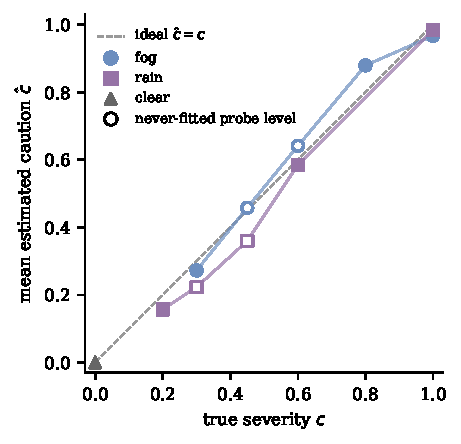
\includegraphics[width=0.78\columnwidth]{figures/fig_estimator_calibration.pdf}
\caption{Estimator calibration on held-out routes: mean $\hat c$ against true severity $c$.}\label{fig:calib}
\end{figure}

\begin{table}[t]
\centering\caption{Held-out estimator results (seeds 9040--9042). Probe levels were never fitted.}\label{tab:est}
\footnotesize
\begin{tabular}{lrrrrr}
\toprule
Condition & Kind recall & $\bar{\hat c}$ & True $c$ & Bias & MAE \\
\midrule
Clear 0 & 1.000 & 0.000 & 0.00 & +0.000 & 0.000\\
Fog 0.3 & 1.000 & 0.272 & 0.30 & $-$0.028 & 0.035\\
Fog 0.45$^\dagger$ & 1.000 & 0.458 & 0.45 & +0.008 & 0.030\\
Fog 0.6$^\dagger$ & 1.000 & 0.641 & 0.60 & +0.041 & 0.046\\
Fog 0.8 & 1.000 & 0.879 & 0.80 & +0.079 & 0.079\\
Fog 1.0 & 1.000 & 0.967 & 1.00 & $-$0.033 & 0.033\\
Rain 0.2 & 0.811 & 0.157 & 0.20 & $-$0.043 & 0.047\\
Rain 0.3$^\dagger$ & 0.883 & 0.223 & 0.30 & $-$0.077 & 0.077\\
Rain 0.45$^\dagger$ & 1.000 & 0.360 & 0.45 & $-$0.090 & 0.090\\
Rain 0.6 & 1.000 & 0.585 & 0.60 & $-$0.015 & 0.023\\
Rain 1.0 & 1.000 & 0.985 & 1.00 & $-$0.015 & 0.015\\
\bottomrule
\end{tabular}
\\[1mm]\footnotesize $^\dagger$ probe level, never used in any fit.
\end{table}

\subsection{Perception under weather (illustrative captures)}
To show how the weather acts on the perception chain, one scene with sparse traffic (density $0.05$) was captured once in clear weather, and every weather setting was then applied to the same raw camera frames with the evaluation's own filter and noise seed. The stereo depth, the detections and the BEV grid were computed for each setting by the unmodified pipeline. Figure~\ref{fig:cams} shows the five camera views, Fig.~\ref{fig:depthw} the front-left frame with detections and the stereo depth map, and Fig.~\ref{fig:bevw} the resulting BEV grids next to the simulator reference. These are single-scene illustrations, not a measured result.
\todo{After the capture run, add one sentence with the measured valid-depth fraction and the number of detections per setting (from capture/stats.json).}
\IfFileExists{figures/fig_camera_views.pdf}{\begin{figure*}[t]\centering\includegraphics[width=0.9\textwidth]{figures/fig_camera_views.pdf}\caption{The five RGB camera views of the captured scene (clear weather).}\label{fig:cams}\end{figure*}}{\begin{figure*}[t]\centering\fbox{\parbox{0.9\textwidth}{\centering\textcolor{blue}{PENDING CAPTURE: five camera views}}}\caption{The five RGB camera views of the captured scene (clear weather).}\label{fig:cams}\end{figure*}}
\IfFileExists{figures/fig_depth_weather.pdf}{\begin{figure*}[t]\centering\includegraphics[width=0.9\textwidth]{figures/fig_depth_weather.pdf}\caption{Same scene under five weather settings. Top: weather-processed front-left frame with YOLOv8n detections. Bottom: stereo SGM depth map (black = no valid depth).}\label{fig:depthw}\end{figure*}}{\begin{figure*}[t]\centering\fbox{\parbox{0.9\textwidth}{\centering\textcolor{blue}{PENDING CAPTURE: weathered frames, detections, depth maps}}}\caption{Same scene under five weather settings: frame with detections and stereo depth map.}\label{fig:depthw}\end{figure*}}
\IfFileExists{figures/fig_bev_weather.pdf}{\begin{figure*}[t]\centering\includegraphics[width=0.9\textwidth]{figures/fig_bev_weather.pdf}\caption{BEV grids built from the camera pipeline for the same scene (ego triangle at row 56, column 32), next to the privileged simulator reference. Colours: free, route centreline, lane boundary, obstacle.}\label{fig:bevw}\end{figure*}}{\begin{figure*}[t]\centering\fbox{\parbox{0.9\textwidth}{\centering\textcolor{blue}{PENDING CAPTURE: BEV grids per weather}}}\caption{BEV grids built from the camera pipeline for the same scene under each weather setting.}\label{fig:bevw}\end{figure*}}


\subsection{Driving results on 20 paired seeds}
Table~\ref{tab:main} and Fig.~\ref{fig:bars} summarise the $120$ completed episodes (seeds $5200$--$5219$, horizon $1600$).

\begin{table*}[t]
\centering\caption{Paired evaluation of Model A (non-adaptive) and Model C (adaptive), 20 paired seeds per condition, horizon 1600. $^{*}$C/O/T: crashes / off-road / timeouts. Success intervals are Wilson $95\%$. Wh/km on both-success pairs is paired; the interval is a seed-level bootstrap of the mean difference.}\label{tab:main}
\footnotesize
\begin{tabular}{llcccccccc}
\toprule
Condition & Model & Success & C/O/T$^{*}$ & Route compl. & Speed (m/s) & Duration (s) & Hard brake & Wh/km (both) & Wh/km (all)\\
\midrule
Clear & A & 20/20 (0.84--1.00) & 0/0/0 & 0.989 & 7.58 & 53.4 & 0.035 & 106.0 & 110.7\\
 & C & 17/20 (0.64--0.95) & 1/0/2 & 0.906 & 7.13 & 59.9 & 0.017 & 97.0 & 109.8\\
 & $\Delta$ & \multicolumn{8}{l}{McNemar $p=0.25$ (3 A-only, 0 C-only); $\Delta e=-9.0$ Wh/km, 95\% CI $[-24.8,+5.2]$, $-8.5\%$ ($n=17$)}\\
\midrule
Fog 1.0 & A & 20/20 (0.84--1.00) & 0/0/0 & 0.989 & 7.82 & 50.8 & 0.027 & 106.8 & 106.8\\
 & C & 20/20 (0.84--1.00) & 0/0/0 & 0.989 & 5.57 & 71.2 & 0.003 & 54.5 & 54.5\\
 & $\Delta$ & \multicolumn{8}{l}{McNemar $p=1.00$; $\Delta e=-52.3$ Wh/km, 95\% CI $[-65.5,-41.1]$, $-48.9\%$ ($n=20$)}\\
\midrule
Rain 1.0 & A & 20/20 (0.84--1.00) & 0/0/0 & 0.989 & 7.82 & 50.8 & 0.027 & 103.4 & 103.4\\
 & C & 20/20 (0.84--1.00) & 0/0/0 & 0.988 & 5.50 & 72.1 & 0.002 & 53.1 & 53.1\\
 & $\Delta$ & \multicolumn{8}{l}{McNemar $p=1.00$; $\Delta e=-50.3$ Wh/km, 95\% CI $[-61.1,-40.4]$, $-48.7\%$ ($n=20$)}\\
\bottomrule
\end{tabular}
\end{table*}

\begin{figure*}[t]
\centering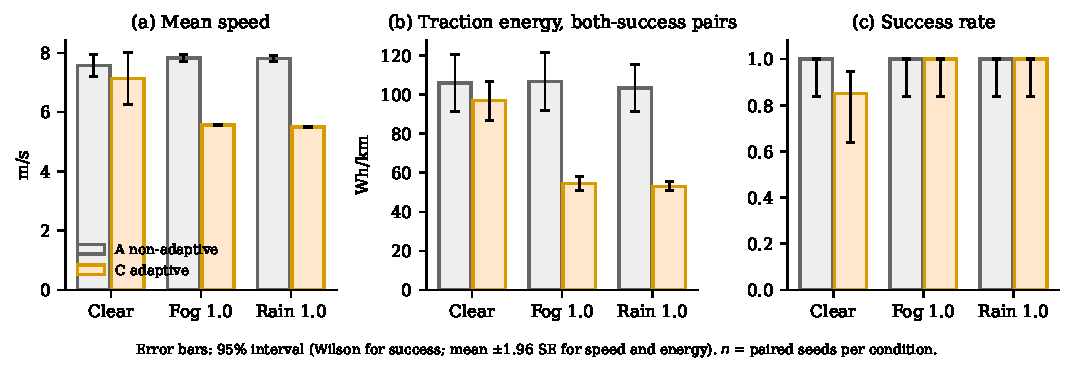
\includegraphics[width=0.92\textwidth]{figures/fig_speed_energy_v2.pdf}
\caption{Mean speed, paired Wh/km (both-success pairs) and success rate per condition, Model A versus Model C ($n=20$ pairs). Error bars are $95\%$ intervals.}\label{fig:bars}
\end{figure*}

Figure~\ref{fig:traces} shows the time course. In fog and rain the estimated caution rises to about $1$ within seconds and Model C settles at about $5.5$\,m/s, whereas Model A holds about $8.3$\,m/s. In clear weather $\hat c$ stays at $0$ and the median speeds coincide; the failures of Section~\ref{sec:clearfail} lie in the lower tail and are not visible in a median.
\begin{figure*}[t]
\centering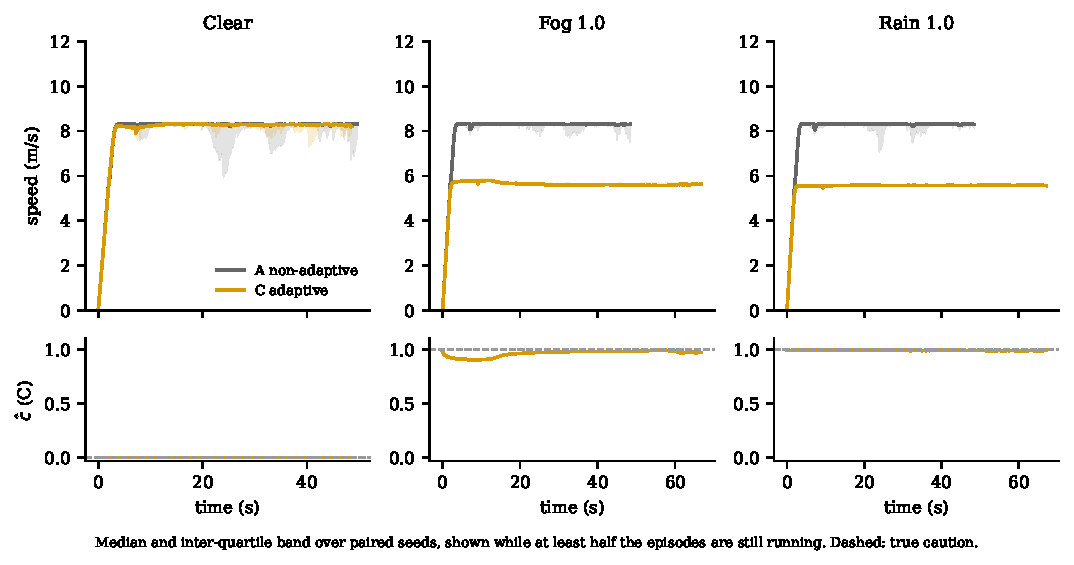
\includegraphics[width=0.85\textwidth]{figures/fig_speed_time.pdf}
\caption{Speed (top) and estimated caution of Model C (bottom) against time. Median and inter-quartile band over the paired seeds, shown while at least half of the episodes are still running. Dashed: true caution.}\label{fig:traces}
\end{figure*}

\textbf{Fog and rain.} In both severe conditions, Model~C and Model~A succeeded in all $20$ episodes with no collision or off-road event. Model~C drove at $5.57$ and $5.50$\,m/s against $7.82$\,m/s for Model~A, close to the teacher's target of $5.56$\,m/s at $c=1$, which is the intended behaviour. Traction energy per kilometre fell from $106.8$ to $54.5$\,Wh/km in fog and from $103.4$ to $53.1$\,Wh/km in rain (paired differences of $-52.3$ and $-50.3$\,Wh/km; $95\%$ intervals $[-65.5,-41.1]$ and $[-61.1,-40.4]$), at the cost of longer episodes ($71$--$72$\,s against $51$\,s). Model~C also braked hard on $0.3\%$ and $0.2\%$ of steps against $2.7\%$ for Model~A, i.e.\ it slows early instead of braking late.

\subsection{Clear weather: where the adaptive policy fails}
\label{sec:clearfail}
In clear weather Model~C succeeded in $17$ of $20$ episodes and Model~A in $20$ of $20$: a gap of $15$ percentage points, outside the $10$-point descriptive margin. Of the $3$ Model~C failures, $1$ was a collision and $2$ were timeouts. The exact McNemar test gives $p=0.25$ ($3$ A-only successes, $0$ C-only), so at this sample size the gap is not statistically established, but we report the point estimate as a failure of the adaptation in clear weather. Mean route completion was $0.906$ for Model~C and $0.989$ for Model~A, and mean speed $7.13$ against $7.58$\,m/s ($6\%$ lower, outside our $5\%$ tolerance). The paired energy difference on the $17$ both-success pairs is $-9.0$\,Wh/km ($-8.5\%$; $95\%$ interval $[-24.8,+5.2]$), which includes zero. Over all episodes the energy per kilometre is practically equal ($110.7$ for A and $109.8$ for C), so we do not claim an energy benefit in clear weather.

\begin{table}[t]
\centering\caption{Model C failures in clear weather. The estimated caution was $0.00$ throughout all three episodes.}\label{tab:fail}
\footnotesize
\begin{tabular}{lllp{3.6cm}}
\toprule
Seed & Outcome & Step & Behaviour (Model A on the same seed)\\
\midrule
5204 & timeout & 177 & cruised at $\approx8.2$\,m/s, braked to a stop, throttle $\approx-0.3$ for $1400$ steps; $27\%$ route (A: finished, $583$ steps)\\
5211 & timeout & 411 & cruised at $8.3$\,m/s, then stopped with throttle $-0.7$ to $-0.8$; $86\%$ route (A: finished, $484$ steps)\\
5214 & collision & 81 & held $7.9$\,m/s into a curve and collided; $19\%$ route (A slowed from $8.2$ to $5.8$\,m/s and steered)\\
\bottomrule
\end{tabular}
\end{table}

\textbf{What the failures are.} Table~\ref{tab:fail} lists the three episodes. In both stalls the car cruised at the target speed, stopped abruptly, and stayed stopped with the brake applied until the horizon. In the third episode it did not slow for a curve that Model~A negotiated. In all three the estimated caution was exactly $0.00$, so the estimator is not the cause: the network received the correct clear-weather input. For the stalled episodes the privileged log of the nearest simulator vehicle ahead in the ego lane within the $17.5$\,m BEV window is empty at every step, so the stalls are not a response to a vehicle that the simulator places in the ego lane inside that window. The log does not cover static obstacles, and we have not yet inspected the BEV grid at the stall step, so we do not know whether the network brakes for a false detection, a map feature or a state it has never seen. We state this as an open question.

\subsection{Horizon sensitivity}
Success at a horizon of $800$ steps (derived from the same traces) separates the two models in adverse weather, because Model~C drives slowly: A succeeds in $19$, $20$ and $20$ of $20$ episodes (clear, fog, rain), C in $17$, $15$ and $14$. The $1600$-step horizon is the primary one; at $800$ steps, the slower driving that saves energy is counted as failure. The choice of time limit therefore matters for how energy-saving behaviour is scored.

\subsection{Extension to 40 paired seeds (EXTENSION)}
\todo{Seeds 5220--5239 are running (same configuration, separate output directory). When complete, pool with the 20-seed snapshot, re-run \texttt{analyze\_severity\_eval.py}, and update Table~\ref{tab:main}, the McNemar test for clear weather, and the conclusions. Do not alter the 20-seed numbers above; report the pooled and the extension-only results separately.}

%==============================================================================
\section{Discussion and Limitations}
\label{sec:limits}
\textbf{Summary.} Model~C demonstrates strong adaptation under severe synthetic fog and rain: it halves traction energy per kilometre without any loss of success or any collision in $20$ paired episodes per condition, and the speed drop matches the teacher's design. Preserving clear-weather performance is an unresolved issue: Model~C lost three of $20$ clear episodes that Model~A completed.

\textbf{Possible causes (hypotheses, not tested).} (i) \emph{DAgger on stopped states}: a student that stops is labelled by a teacher that also brakes in the stopped state, so the data can reinforce a stop; a stalled student visited this state in training rounds as well. (ii) \emph{Training mix}: clear weather is $25\%$ of the training steps ($5{,}797$ of $23{,}532$) and the schedule used $12$ episodes per round against $40$ planned, so full-speed clear driving with traffic is under-represented. (iii) \emph{Plug-in training}: the network was trained with oracle caution; the clear-weather input $\chat=0$ is the same value, so the plug-in is not a plausible cause for these three episodes. We did not retrain, change the model, or select checkpoints after seeing the results.

\textbf{Limitations.}
\begin{itemize}
\item \emph{Synthetic image-space weather.} The fog and rain filters have no depth dependence and no extinction coefficient. The estimator therefore largely recovers the filter's own setting, and its accuracy is an upper bound for real weather. Nothing here shows transfer to real fog or rain.
\item \emph{Identity caution is an assumption.} Equal fog and rain levels are not equally dangerous, and the teacher's speed rule is a design choice, not a visibility-derived bound.
\item \emph{Pilot scale.} $20$ pairs per condition gives wide intervals (a $20/20$ result has a Wilson lower bound of $0.84$) and cannot support a non-inferiority claim. Only large effects, such as the energy difference in fog and rain, are detectable. The held-out estimator set is three routes.
\item \emph{Reduced training schedule.} $12$ episodes per round and $4$ rounds, final-round checkpoint, no validation-based selection.
\item \emph{Only two severity extremes were driven.} Driving was evaluated at $c=0$ and $c=1$ only. Intermediate levels (fog $0.6$, rain $0.45$) were reserved but not evaluated, so monotone behaviour across severity is shown only for the teacher and in the training data, not in closed-loop evaluation.
\item \emph{Energy is mechanical traction work} for a declared virtual vehicle, with no regeneration, drivetrain or auxiliary losses and flat roads. Slower driving lowers aerodynamic work, so a large part of the saving is a property of speed; the claim is about \emph{selective} slowing, which holds only if clear-weather behaviour is preserved, which is exactly what fails here.
\item \emph{Time limit.} Slower driving means longer trips; at an $800$-step limit the adaptive policy would fail more often.
\item \emph{Simulation only}, sparse traffic (density $0.05$), one map family.
\end{itemize}

%==============================================================================
\section{Conclusion}
A camera-image severity estimate, passed as a single caution scalar to a camera-trained driving policy, makes the vehicle drive about $30\%$ slower and use about $49\%$ less traction energy per kilometre in severe synthetic fog and rain, with unchanged success and no collisions in $20$ paired episodes per condition. The same system fails in $3$ of $20$ clear-weather episodes in which the non-adaptive policy succeeds, with correct zero caution. This is the main open problem: selective adaptation requires that clear-weather behaviour be preserved. The evaluation is pilot-scale and synthetic; the extension to $40$ seeds and a diagnosis of the clear-weather stalls are the next steps.

\section*{Reproducibility}
Code lives in \texttt{bev\_rl/adaptive/}. The $20$-seed results are the frozen snapshot with a SHA-256 manifest (\texttt{severity\_eval\_20seed\_snapshot}). The analysis is \texttt{analyze\_severity\_eval.py}. The pre-registration amendment and change log record every deviation (episodes per round, reduced rounds, evaluation order).

\appendices
\section{Module Expansions}\label{app:modules}
Figures~\ref{fig:app_est}--\ref{fig:app_train} expand the modules of Fig.~\ref{fig:arch}. Orange marks what is new in this work; dashed boxes are used only for training.
\begin{figure}[t]
\centering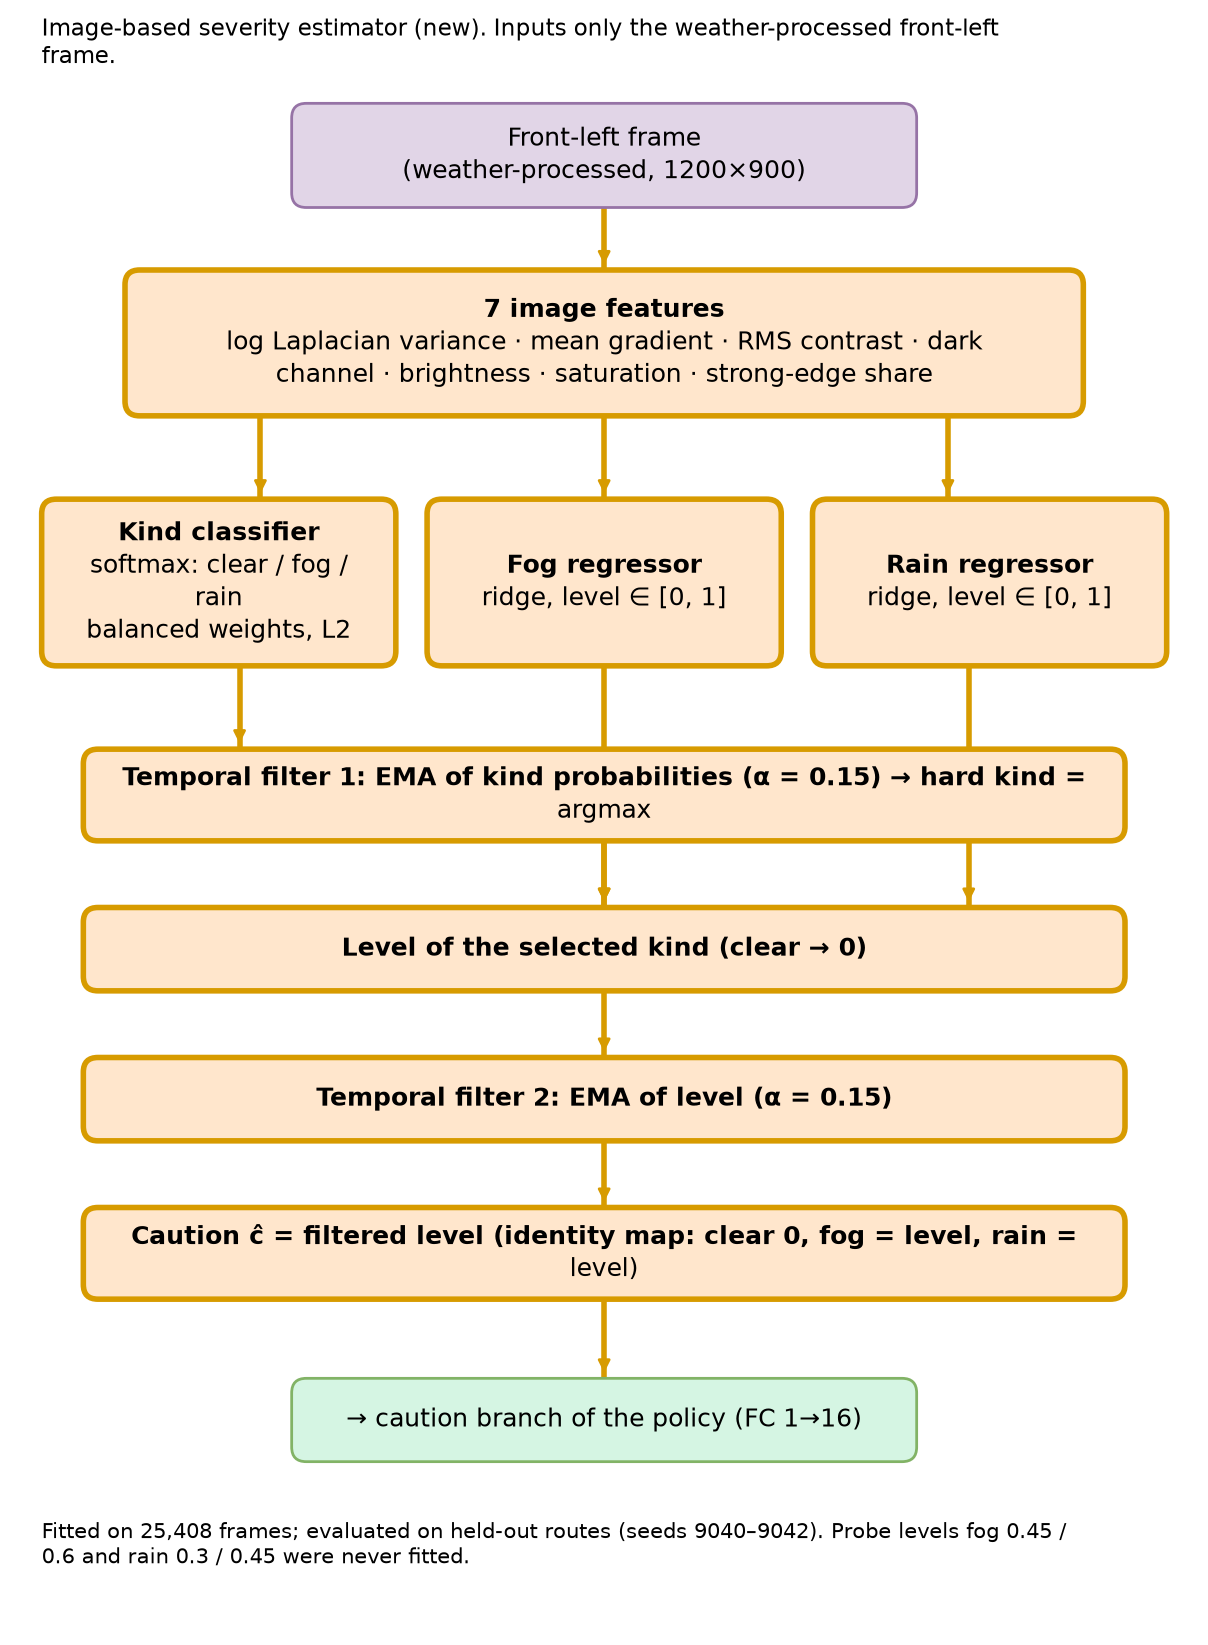
\includegraphics[width=0.92\columnwidth]{figures/fig_arch_estimator.png}
\caption{Severity estimator: seven image features, a kind classifier and two level regressors, followed by two temporal filters and the identity caution map.}\label{fig:app_est}
\end{figure}
\begin{figure}[t]
\centering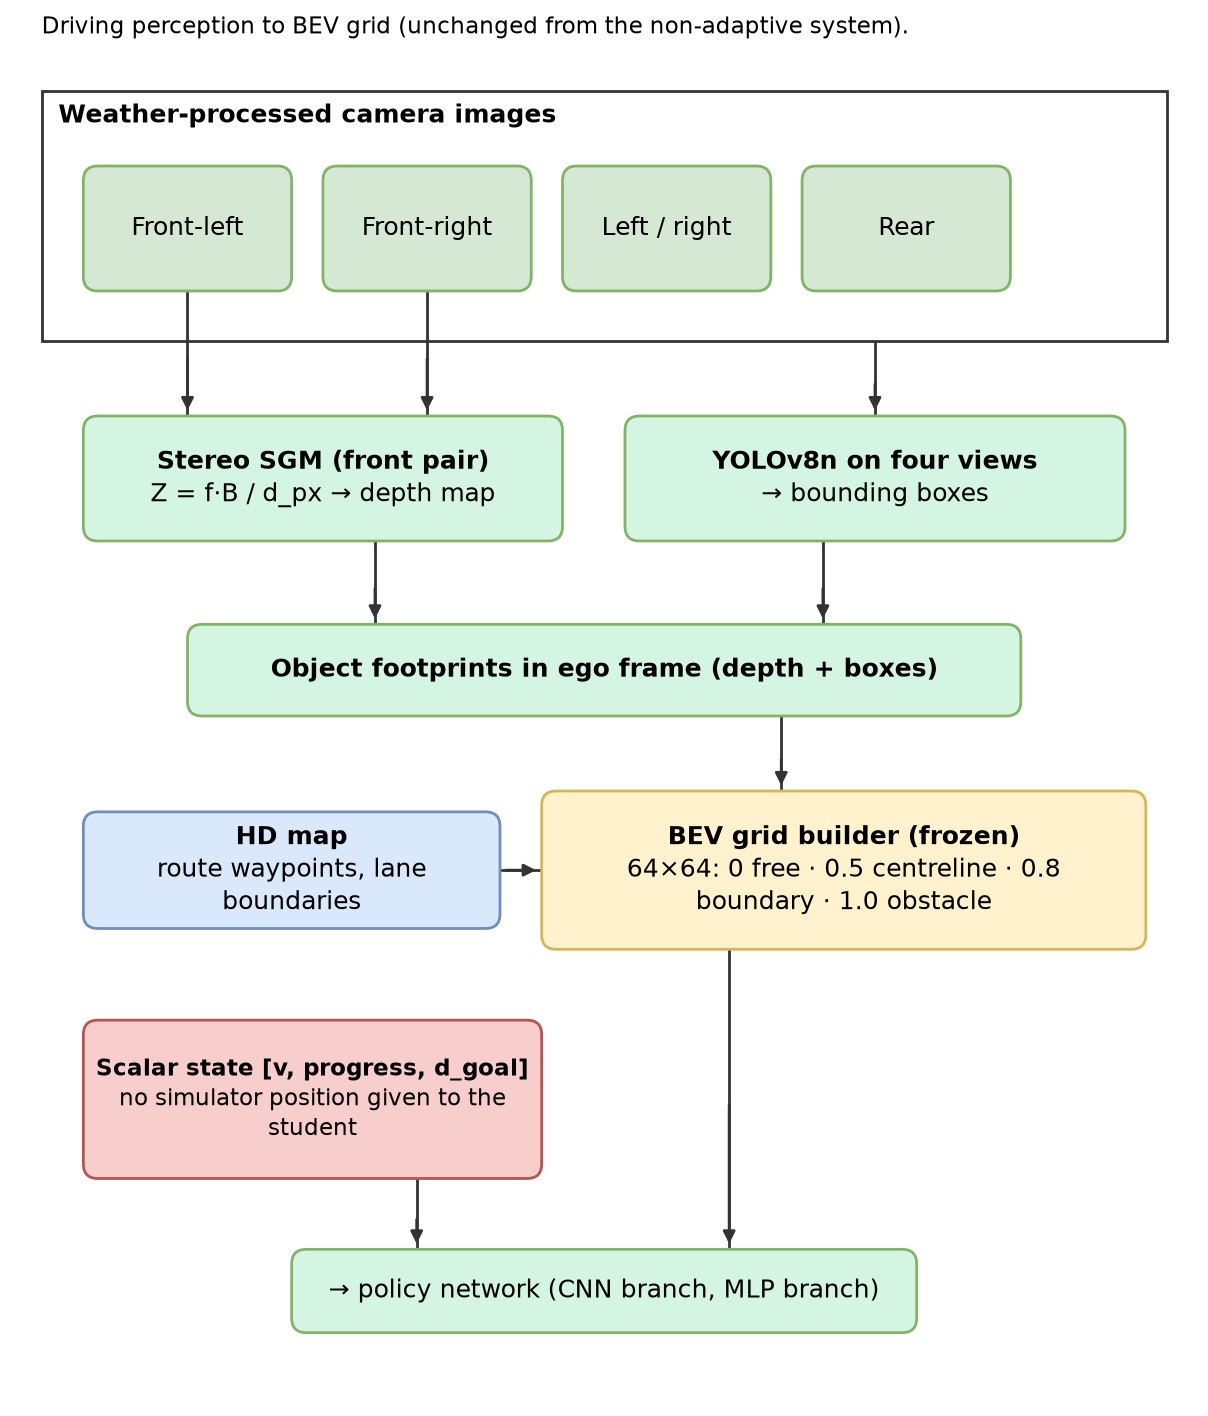
\includegraphics[width=0.92\columnwidth]{figures/fig_arch_perception.png}
\caption{Driving perception to the BEV grid (shared by Models A and C).}\label{fig:app_perc}
\end{figure}
\begin{figure}[t]
\centering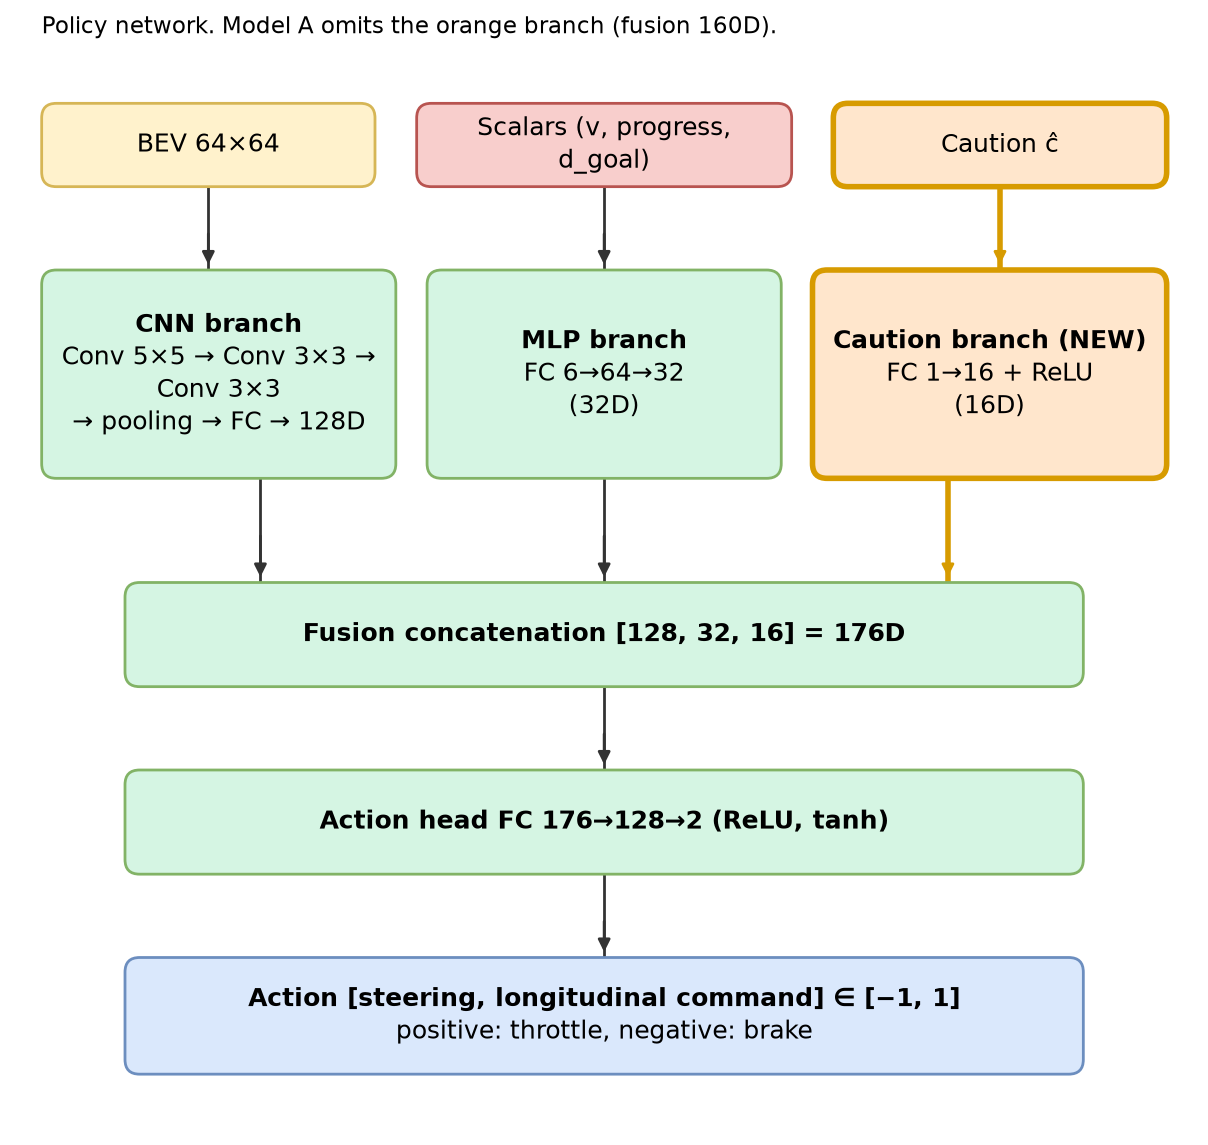
\includegraphics[width=0.92\columnwidth]{figures/fig_arch_policy.png}
\caption{Policy network. Model A omits the caution branch (160-D fusion).}\label{fig:app_pol}
\end{figure}
\begin{figure}[t]
\centering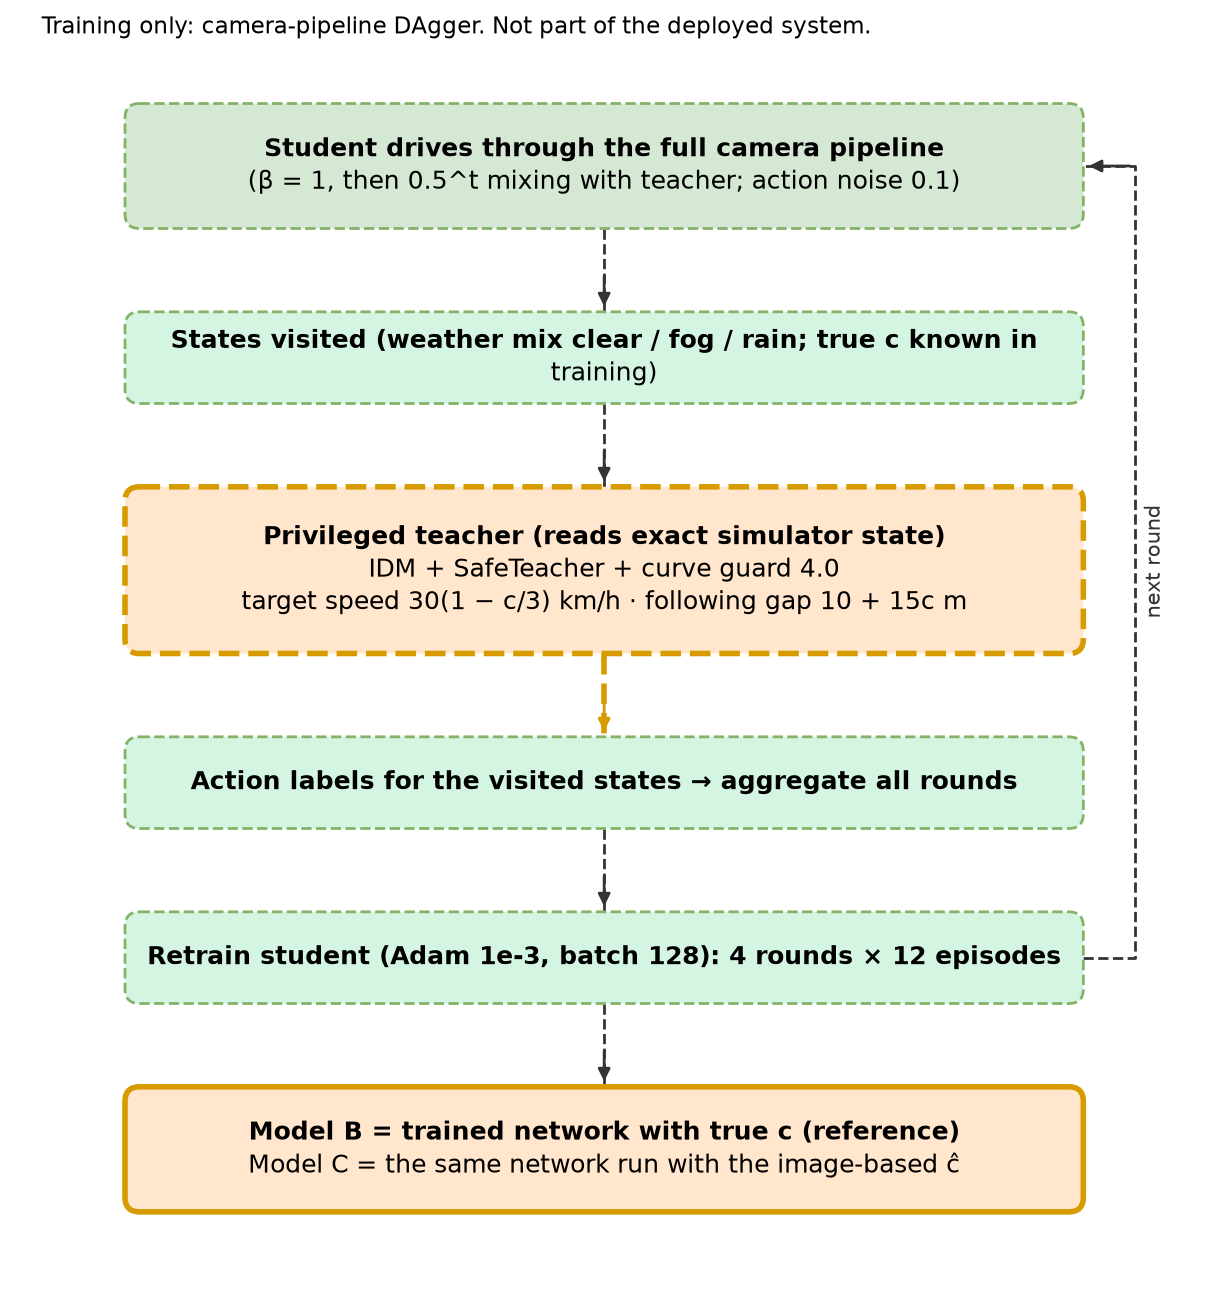
\includegraphics[width=0.92\columnwidth]{figures/fig_arch_training.png}
\caption{Camera-pipeline DAgger (training only).}\label{fig:app_train}
\end{figure}

\bibliographystyle{IEEEtran}
\bibliography{references}
\end{document}
